% Tikz File 'model640.tex'
\documentclass{standalone}
\usepackage{tikz} %Graphics
\usepackage{pgfplots} % XY plots

%\usetikzlibrary{...}
\begin{document}
	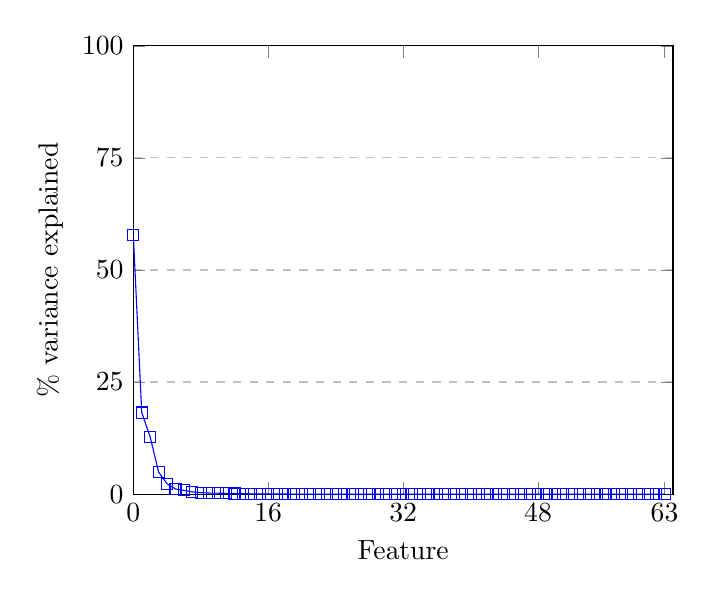
\begin{tikzpicture}
		\begin{axis}[
		%title={Receptive field vs Layer},
		xlabel={Feature},
		ylabel={\% variance explained},
		xmin=0, xmax=64,
		ymin=0, ymax=100,
		xtick={0,16,32,48,63},
		ytick={0,25,50,75,100},
		legend pos=north west,
		ymajorgrids=true,
		grid style=dashed,
		]
		
		\addplot[
		color=blue,
		mark=square,
		]
		coordinates {
			(0,57.791)(1,18.194)(2,12.753)(3,4.917)(4,2.322)(5,1.154)(6,0.849)(7,0.491)
			(8,0.326)(9,0.242)(10,0.211)(11,0.172)(12,0.136)(13,0.108)(14,0.067)(15,0.061)
			(16,0.05)(17,0.029)(18,0.022)(19,0.015)(20,0.012)(21,0.011)(22,0.008)(23,0.007)
			(24,0.006)(25,0.005)(26,0.005)(27,0.004)(28,0.003)(29,0.003)(30,0.003)(31,0.003)
			(32,0.002)(33,0.002)(34,0.002)(35,0.001)(36,0.001)(37,0.001)(38,0.001)(39,0.001)
			(40,0.001)(41,0.001)(42,0.001)(43,0.001)(44,0.001)(45,0.001)(46,0.)(47,0.)(48,0.)
			(49,0.)(50,0.)(51,0.)(52,0.)(53,0.)(54,0.)(55,0.)(56,0.)(57,0.)(58,0.)(59,0.)
			(60,0.)(61,0.)(62,0.)(63,0.)
		};
		%\legend{CuSO$_4\cdot$5H$_2$O}
		
		\end{axis}
	\end{tikzpicture}
\end{document}
